%%%%%%%%%%%%%
%  Ch1 : Generalities  %
%%%%%%%%%%%%%

\chapter{Generalities}
\section{Fundamental laws}
\subsubsection{Reminder}
	Let's first remind the 3 basic principles of \textit{Fluid mechanics I} : \\
	
	\begin{itemize}
		\item[•] \textbf{Mass conservation :} \textit{The mass of a closed system remains constant in time.}\\
		This is much a definition of a closed system than a principle. We have to notice that related to Einstein law of relativity, $E = mc^2$, mass must vary with energy. But if we exclude nuclear reactions, our approximation is valid. Indeed, the square of light velocity has a greater impact on energy than the mass term. If the energy exchange is huge like in nuclear reaction, mass vary, but in smaller energies domain (combustion for example), the mass can be considered as constant. \\
		
		\item[•] \textbf{Newton's law :} \textit{the time rate of change of momentum of a closed system is equal to the sum of the forces applied on the system.} \\
		
		\item[•] \textbf{First principle of thermodynamics :} \textit{the time rate of change of the total energy of a closed system is equal to the sum of the power of the forces applied on the system and the thermal power provided to the system.}
	\end{itemize}		
	
	\subsubsection{Useful equations}
	
	\begin{wrapfigure}[9]{l}{4cm}
	\vspace{-5mm}
	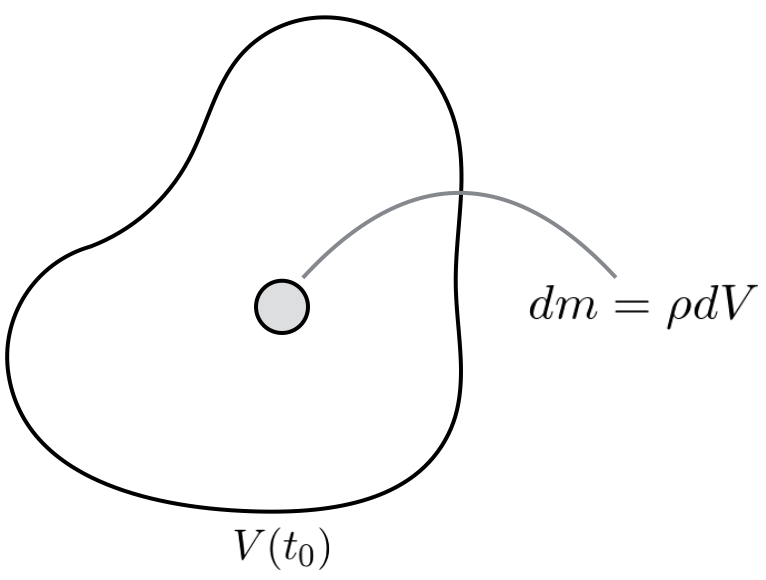
\includegraphics[scale=0.3]{ch1/1}
	\captionof{figure}{}
	\label{fig:1.1}
	\end{wrapfigure}
	Let's consider the integral on a moving volume of a function depending on time and position $f(\vec{x},t)$. Imagine that \autoref{fig:1.1} represents the moving volume at initial time containing mass $m$. An infinitesimal part of that volume contains an infinitesimal mass $dm = \rho dV$, where $\rho$ is mass density. We deduce the expression of the total mass at any time by that of the initial time  
	\begin{equation}
		M(t_0) = \int _{V(t_0)}\rho (\vec{x},t_0)\, dV \qquad \Rightarrow M(t) = \int _{V(t)}\rho (\vec{x},t)\, dV
	\end{equation}
	By considering $\rho (\vec{x},t)$ as $f(\vec{x},t)$, the derivative of the integral is given by
	
	\begin{center}
	\theor{\textbf{Reynolds transport theorem}
	\begin{equation}
		\frac{d}{dt}\int _{V(t)}f (\vec{x},t)\, dV = \int _{V(t)} \frac{\D f}{\D t} (\vec{x},t)\, dV + \oint _{S(t) = \D V(t)} f(\vec{x},t) \vec{b}\, \vec{n}\, dS
	\end{equation}
	where $\vec{b}$ is the surface displacement velocity. }
	\end{center}
	
	The second equation that will be used in the developement is given by
	\begin{center}
	\theor{\textbf{Gauss theorem}
	\begin{equation}
		\oint _{S = \D V} \vec{a} \, \vec{n} \, dS = \int _V \nabla \vec{a}\, dV
	\end{equation}}
	\end{center}
	
	\subsection{Mass conservation equation}
	If $V(t)$ is the moving volume occupied by the closed system as time varies, then by definition of a closed system $\frac{dM(t)}{dt} = 0$. The corresponding equation using Reynolds transport theorem is 
	\begin{equation}
		M(t) = \int _{V(t)} \rho\, dV \qquad \Rightarrow \frac{dM(t)}{dt} = \int _{V(t)} \frac{\D \rho}{\D t}\, dV + \oint _{S(t) = \D V(t)} \rho\, \vec{b}\, \vec{n}\, dS = 0
	\end{equation}
	\begin{wrapfigure}[9]{l}{3cm}
	\vspace{-5mm}
	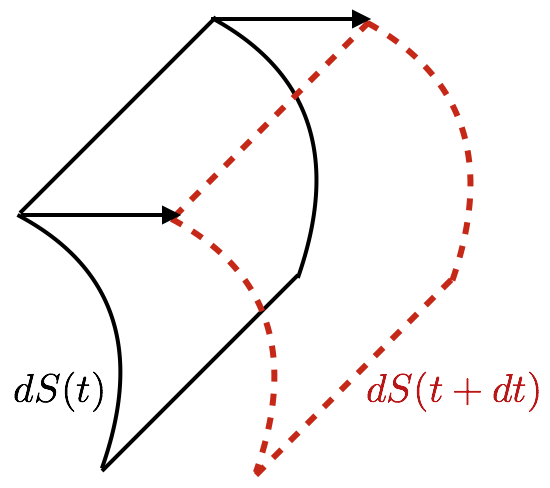
\includegraphics[scale=0.3]{ch1/2}
	\captionof{figure}{}
	\label{fig:1.2}
	\end{wrapfigure}
	We have to express that this volume is not traversed by material. There is no flux of fluid and the particles in the volume are always the same. By definition, the infinitesimal distance traveled by the surface and the fluid are
	\begin{equation}
		d\vec{x} = \vec{b}\, dt \qquad and \qquad d\vec{x}' = \vec{u}\, dt
	\end{equation}	 
	where $\vec{u}$ is the fluid velocity. Under wich condition do we know that the fluid has not traversed the boundary? We have to define the relative dispolacement $d\vec{x}'-d\vec{x}$ of the fluid in regard to the fluid. For a closed system 
	\begin{equation}
	\begin{aligned}
		(d\vec{x}'-d\vec{x})\cdot \vec{n} = 0 \quad &\Leftrightarrow \quad dt (\vec{u}-\vec{b})\cdot \vec{n} = 0 \quad \Leftrightarrow \quad (\vec{u}-\vec{b})\cdot \vec{n} = 0 \\
		&\Rightarrow \quad \vec{b} \vec{n} = \vec{u} \vec{n}
		\end{aligned}
	\end{equation}
	\begin{center}
	\theor{\textbf{Mass conservation equation for closed systems (integral form)}
	\begin{equation}
		\int _{V(t)} \frac{\D \rho}{\D t}\, dV + \oint _{S(t) = \D V(t)} \rho\, \underbrace{\vec{b}\, \vec{n}}_{=\vec{u}\, \vec{n}}\, dS =0
		\label{eq:1.7}
	\end{equation}}
	\end{center}
	
	How to write this equation in a different way? Let's consider now a fixed open system composed of fluid particles in the fixed volume $V_0(t) = V(t_0)$. Similarly to the previous point, the mass variation in this fixed volume is expressed like 
	\begin{equation}
		M_0(t) = \int _{V_0(t)} \rho\, dV \qquad 
		\Rightarrow \int _{V_0(t)} \frac{\D \rho}{\D t}\, dV + \oint _{S_0(t) = \D V_0(t)} \rho\, \vec{b}\, \vec{n}\, dS.
	\end{equation}
	The volume integral expresses the variable mass in the fixed volume and the surface integral is nul due to the nul surface velocity (since the volume is fixed). This relation enables us to write the 
	\begin{center}
	\theor{\textbf{Mass conservation equation for fixed open systems (integral form)}
	\begin{equation}
		\frac{dM_0}{dt} + \underbrace{\oint _{S_0(t) = \D V_0(t)} \rho\, \vec{u}\, \vec{n}\, dS = 0}_{\mbox{mass flow out of the system}}
	\end{equation}}
	\end{center}	
	Let's finally consider an arbitrary open system containing fluid particles in a moving volume $V_*(t)$ such that $V_*(t_0) = V(t_0) = V_0$. Similarly we have using the Reynolds transport theorem
	\begin{equation}
		M_*(t) = \int _{V_*(t)} \rho\, dV \qquad \Rightarrow \frac{dM_*(t)}{dt} = \int _{V_*(t)} \frac{\D \rho}{\D t}\, dV + \oint _{S_*(t) = \D V_*(t)} \rho\, \vec{b}\, \vec{n}\, dS
	\end{equation}
	Using the definition of the volume at $t=t_0$, we can equalize the volume integral with that of \autoref{eq:1.7} to find 
	\begin{center}
	\theor{\textbf{Mass conservation equation for arbitrary open systems (integral form)}
	\begin{equation}
		\frac{dM_*(t_0)}{dt} + \oint _{S(t_0) = \D V(t_0)} \rho (\vec{u}-\vec{b})\, \vec{n}\, dS = 0
	\end{equation}}
	\end{center}	
	
	Let's now take \autoref{eq:1.7} again and apply Gauss theorem
	\begin{equation}
	\begin{aligned}
		\int _{V(t)} \frac{\D \rho}{\D t}\, dV + \oint _{S(t) = \D V(t)} \rho \underbrace{\vec{u}\, \vec{n}}_{\vec{a}}\, &dS =0 \qquad with \qquad 
		\oint _{S(t)} \rho\, \underbrace{\vec{u}\, \vec{n}}_{\vec{a}}\, dS = \int _{V(t)} \nabla \rho \vec{u} \, dV \\
		&\Leftrightarrow \int _{V(t)} \left[ \frac{\D \rho}{\D t} + \nabla \rho \vec{u} \right] \,dV = 0
		\end{aligned}
	\end{equation}
	For this last equation to be true for all systems, the integrated term must be equal to zero 
	\begin{center}
	\theor{\textbf{Mass conservation equation (differential form (1) - divergent form)}
	\begin{equation}
		\frac{\D \rho}{\D t} + \nabla \rho \vec{u} = 0
		\label{eq:1.13}
	\end{equation}}
	\end{center}
	
	\begin{wrapfigure}[4]{l}{4cm}
	\vspace{-5mm}
	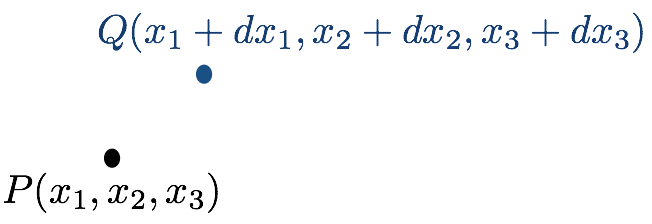
\includegraphics[scale=0.35]{ch1/3}
	\captionof{figure}{}
	\label{fig:1.3}
	\end{wrapfigure}
	In order to find the second differential form, let's consider 2 points Q and P as described in \autoref{fig:1.3}. The difference of density between the 2 points is \\\\\\
	\begin{equation}
	\begin{aligned}
		\rho _Q(t+dt) - \rho _P(t) &= \rho (x_1+dx_1,x_2+dx_2,x_3+dx_3,t+dt) - \rho (x_1,x_2,x_3)  \\
		&= d\rho = \frac{\D \rho}{\D x_1}dx_1 + \frac{\D \rho}{\D x_2}dx_2 + \frac{\D \rho}{\D x_3}dx_3 + \frac{\D \rho}{\D t}dt
		\end{aligned}
		\label{eq:1.14}
	\end{equation}
	In general, the fluid particles at $P(t)$ and $Q(t+dt)$ are different. However, if $dx_1 = u_1 dt, dx_2 = u_2 dt, dx_3 = u_3 dt$, then the fluid particles at the 2 points are the same. By making appear these velocities in \autoref{eq:1.14}, 
	\begin{equation}
		d\rho = \left( \frac{\D \rho}{\D x_1}u_1 + \frac{\D \rho}{\D x_2}u_2 + \frac{\D \rho}{\D x_3}u_3 + \frac{\D \rho}{\D t}\right) dt
	\end{equation}
	Finally, after dividing by $dt$ the 2 members of the equation, we obtain the definition of the time rate of change of density when I follow the fluid $\dot{\rho}$. As \autoref{eq:1.13} can be expressed in term of indicial notation like 
	\begin{equation}
		\frac{\D \rho}{\D t} + u_i \frac{\D\rho}{\D x_i} + \rho \frac{\D u_i}{\D x_i} = 0 
	\end{equation}
	Replacing the sum of first and second term by $\dot{\rho}$ gives the last form
	\begin{center}
	\theor{
	\textbf{Mass conservation equation (differential form (2) - substancial form)}
	\begin{equation}
	\dot{\rho} + \rho \nabla \vec{u} = 0
	\label{eq:1.17}
	\end{equation}
	}
	\end{center}
	
	\subsection{Newton's second law : Momentum equation}
	\begin{wrapfigure}[8]{l}{4cm}
	\vspace{-5mm}
	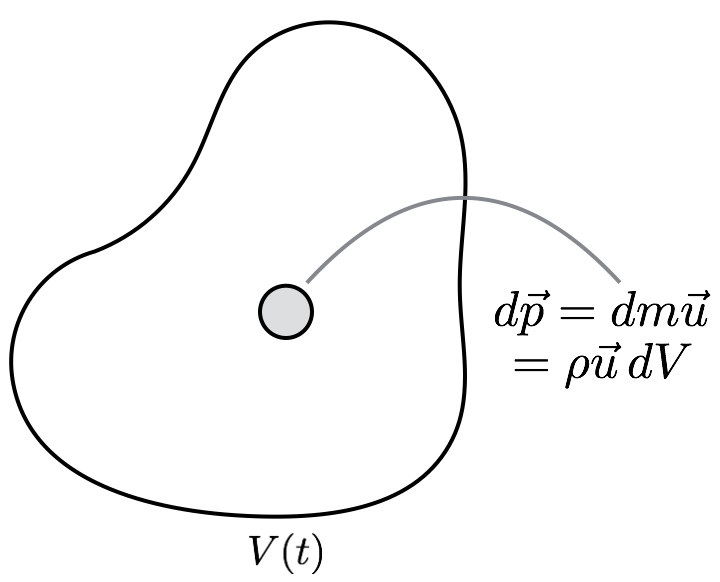
\includegraphics[scale=0.3]{ch1/4}
	\captionof{figure}{}
	\label{fig:1.4}
	\end{wrapfigure}
	Momentum in this course is noted $\vec{P}(t)$. For closed systems,
	\begin{equation}
		\frac{d\vec{P}(t)}{dt} = \sum \vec{F} = \frac{d}{dt}\int _{V(t)} \rho \vec{u}\, dV
		\label{eq:1.18}
	\end{equation}
	where $\rho \vec{u}$ is the momentum density. We will spell out the expression of the 2 members. First, the derivative, using the Reynolds transport theorem gives 
	\begin{equation}
		\frac{d\vec{P}}{dt} = \int _{V(t)} \frac{\D \rho \vec{u}}{\D t}\, dV + \oint _{S(t) = \D V(t)} \rho \vec{u} (\vec{u} \vec{n}) \, dS
	\end{equation}
	This written in indicial notation
	\begin{equation}
	\begin{aligned}
		\frac{dP_i}{dt} &= \int _{V(t)} \frac{\D \rho u_i}{\D t}\, dV + \oint _{S(t) = \D V(t)} \underbrace{\rho u_i u_j}_{tensor :\, \vec{u} \otimes \vec{u}} n_j \, dS\\
		&= \int _{V(t)} \frac{\D \rho u_i}{\D t}\, dV + \oint _{S(t) = \D V(t)} \rho (\vec{u} \otimes \vec{u}) \vec{n}\, dS 
		\end{aligned}
	\end{equation}
	and by applying Gauss theorem to the surface integral

	\begin{center}
	\begin{equation}
		\frac{d\vec{P}}{dt} = \int _{V(t)} \left[\frac{\D \rho \vec{u}}{\D t} + \nabla \rho \vec{u} \otimes \vec{u} \right] dV \qquad and \qquad \frac{dP_i}{dt} = \int _{V(t)} \left[ \frac{\D \rho u_i}{dt} + \frac{\D}{\D x_j} (\rho u_i u_j) \right] dV
	\end{equation}
	\end{center}
	
	Based on the previous forms, we can generalize this for any arbitrary function $\phi$
	\begin{equation}
	\begin{aligned}
		\frac{d}{dt} \int _{V(t)} \rho \phi\, dV  &= \int _{V(t)} \left[\frac{\D \rho \phi}{\D t} + \frac{\D}{\D x_j} \rho \phi u_j \right] dt \\
		&= \int _{V(t)} \left[ \rho \frac{\D \phi}{dt} + \phi \right. \underbrace{\left( \frac{\D \rho}{\D t} + \frac{\D \rho u_j}{\D x_j} \right)}_{= 0\ \autoref{eq:1.13}}\left. + \rho u_j\frac{\D \phi}{\D x_j} \right] dV \\
		&= \int _{V(t)} \rho \left[ \frac{\D \phi}{\D t} + u_j \frac{\D \phi}{\D x_j} \right] dV
	\end{aligned}
	\end{equation}
	Similarly to thermodynamics courses, we can introduce an extensive variable $\Phi$ and an intensive $\phi$ to have 
	\begin{center}
	\theor{
	\textbf{General relation for any arbitrary function in closed systems}
	\begin{equation}
		\frac{d\Phi }{dt} = \int _{V(t)} \left[ \frac{\D \rho \phi}{\D t} + \nabla \rho \phi \vec{u} \right] dV = \int _{V(t)} \rho \dot{\phi} \, dV
	\end{equation}
	}
	\end{center}
	For the specific case where $\Phi = \vec{P}$ and $\phi = \vec{u}$, we obtain
	\begin{equation}
		\frac{d\vec{P}}{dt} = \int _{V(t)} \rho \underbrace{\left[ \frac{\D \vec{u}}{\D t} + \vec{u} \nabla \vec{u} \right]}_{\dot{u}} dV 
		\label{eq:1.24}
	\end{equation}
	We can now express the forces applied on the system. There are 2 main classes : \\
	\begin{itemize}
		\item[•] \textbf{Distance forces (volume)} $\vec{F}_V$ : \\
		This type of force allows a body to influence another without being in contact with. 
		\begin{itemize}
			\item The most present one is gravity which is applied on each fluid particles ($d\vec{F} = dm \vec{g}$). We can imagine that there exists a force density $\vec{f}$ such that 
		\begin{equation}
			\vec{F}_V = \int _{V(t)} \vec{f} \, dV = \int _{V(t)} \rho \vec{a} \, dV
			\label{eq:1.25}
		\end{equation}
		where $\vec{a}$ is a force per unit mass, so an acceleration (gravity : $\vec{f} = \rho \vec{g}$). 
		
			\item If we have an electric material, we can talk about electromagnetic forces, which can be modelled as 
		\begin{equation}
			\vec{f} = \rho _c (\vec{E}+\vec{u}\times \vec{B}) + \vec{J}\times \vec{ B}
		\end{equation}
		where $\rho _c$ is the charge density $[C/m^3]$ and the second term is the Lorentz force. Indeed, if we have a lot of particles, we can talk of an average velocity $\vec{v}_k = \vec{u}+\vec{C}_k$, where $C_k$ is a particular velocity due to molecular agitation.  The force applied on the system is 
		\begin{equation}
			\vec{F}_k = q_k [\vec{E} + \vec{v}_k \times \vec{B}] \qquad \Leftrightarrow \qquad \underbrace{\frac{\sum \vec{F}_k}{V}}_{\rho _c} = \frac{\sum q_k}{V} (\vec{E}+\vec{u}\times \vec{B}) + \underbrace{\frac{\sum q_k \vec{C}_k}{V}}_{\vec{J}} \times \vec{B}
		\end{equation}
		Mollecules are in general neutral, but containing non-neutral regions. Fluids are essentially neutral, $\vec{F}_V = 0$ in most cases. They are called quasi-neutral fluids. Electric influenced fluids will not be considered in that course but they existence has to be known. 
		
			\item They are also entrainment and Coriolis forces in rotating frame of references. These forces due to the rotation of Earth are not considered due to the small rotative velocity, unlike pomps and turbines. \\
		\end{itemize}
		\item[•] \textbf{Contact forces (surface)} $\vec{F}_S$ : \\
		
		\begin{minipage}{0.23\textwidth}
		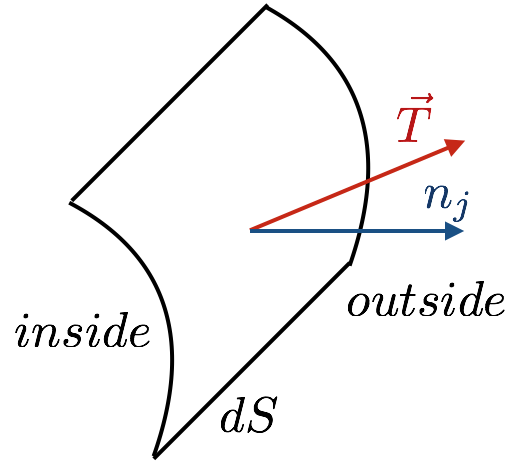
\includegraphics[scale=0.3]{ch1/5}
		\captionof{figure}{ }
		\label{fig:1.5}
		\end{minipage}
		\begin{minipage}{0.7\textwidth}
		These forces results from the contact of an internal and external fluid in regard of a region of surface $dS(t)$. We have 
		\begin{equation}
			d\vec{F}_S = \vec{T}\, dS \qquad \Rightarrow \vec{F}_S = \oint _S \vec{T}\, dS
			\label{eq:1.28}
		\end{equation}
		$\vec{T}$ is a force per unit area, a continuous function of space depending on location $\vec{x}$ and also linearly on the infinitesimal surface orientation $\vec{n}$. If $\vec{T}$ is the force per unit area for a surface element normal
		\end{minipage}
		 to the unit vector in the $j$ direction $e_j$, $\vec{T}(\vec{x}) = \vec{T}_jn_j$. \autoref{eq:1.28} becomes
		 \begin{equation}
		 \vec{F}_S = \oint _S \vec{T}_j n_j \, dS \qquad and \qquad F_{S_i} = \oint _S \underbrace{\tau _{j,i}}_{\sigma _{ji}} n_j\, dS 
		 \label{eq:1.29}
		 \end{equation}
		 where $\sigma _{ji}$ is the stress tensor. 
		\end{itemize}
		We can now take \autoref{eq:1.18} and replace the terms using \autoref{eq:1.24}, \autoref{eq:1.25} and \autoref{eq:1.29} to obtain the 
		
		\begin{center}
		\theor{\textbf{Momentum equation (integral form)}
		\begin{equation}
			\frac{dP_i}{dt} = \int _{V(t)} \left[\frac{\D \rho u_i}{\D t} + \nabla \rho u_i \vec{u} \right] dV = \int _{V(t)} \rho \dot{u}\, dV = \int _{V(t)} \rho a_i\, dV + \oint _{S(t)} \sigma _{ji} n_j \, dS
			\label{eq:1.30}
		\end{equation}
		}
		\end{center}
		We can see that $\sigma _{ji}$ and $\rho u_iu_j$ have the same mathematical nature. This is not surprising because in fact these forces result from molleculare agitation in fluids. Let's discuss it. We said that $\vec{v}_k = \vec{u} + \vec{C}_k$. Let's consider a surface element and make the hypothesis that the fluid is in rest, so the average velocity $\vec{u} = 0$. It doesn't mean that the particles are immobile, but that if all particles have the same mass (pure fluid) and if a certain number of particles are going from right to left with velocity $\vec{c}$, there are the same number of particles going from left to right with velocity $-\vec{c}$. There is no global mass flux. So for n particles going in one direction, the mass flux
		\begin{equation}
			2nm\vec{u} = nm\vec{c} + 2nm(-\vec{c}) = 0 
		\end{equation}
		To obtain the momentum in direction $x_1$, we have to multiply the mass flow in this direction by the velocity in this direction 
		\begin{equation}
			nm (\vec{c}\cdot \vec{e_1})c_1 + nm (-\vec{c_1}\cdot \vec{e_1})(-c_1) = 2nmc_1^2
		\end{equation}
		The global momentum flux traversing the unit surface is so positive going out of the volume. We need so a balance force in the opposite direction to keep the mass in. This explains the presence and nature of $\sigma _{ji}$ which is a momentum flux. \\
	Let's finally establish the differential form of the momentum equation, applying Gauss theorem to the second right side of \autoref{eq:1.30}
	\begin{equation}
		\int _{V(t)} \rho a_i\, dV + \oint _{S(t)} \sigma _{ji} n_j \, dS = \int _{V(t)} \left[ \rho a_i + \frac{\D \sigma _{ji}}{\D x_j} \right] dV
	\end{equation}
	and by considering the whole equation
	\begin{equation}
		\int _{V(t)} \left[ \frac{\D \rho u_i}{\D t} + \frac{\D \rho u_i u_j}{\D x_j} - \rho a_i - \frac{\D \sigma _{ji}}{\D x_j} \right] dV = 0 = \int _{V(t)} \left[ \rho \dot{u}_i - \rho a_i - \frac{\D \sigma _{ji}}{\D x_j} \right] dV
	\end{equation}
	and for this to be true for all systems we consider, we obtain
	\begin{center}
		\theor{\textbf{Momentum equation (differential form (1) - divergent form)}
		\begin{equation}
			\frac{\D \rho u_i}{\D t} + \frac{\D \rho u_i u_j}{\D x_j} = \rho a_i + \frac{\D \sigma _{ji}}{\D x_j} \qquad and \qquad \frac{\D \rho \vec{u}}{\D t} + \nabla \rho \vec{u}\otimes \vec{u} = \rho \vec{a} + \nabla \bar{\bar{\sigma}}
			\label{eq:1.35}
		\end{equation}
		}
		\end{center}
		
	\begin{center}
		\theor{\textbf{Momentum equation (differential form (2) - substancial form)}
		\begin{equation}
			\rho a_i + \frac{\D \sigma _{ji}}{\D x_j} = \rho \dot{u}_i \qquad and \qquad \rho \vec{a} + \nabla \bar{\bar{\sigma}} = \rho \dot{\vec{u}}
			\label{eq:1.36}
		\end{equation}
		}
		\end{center}
		
	\subsection{Angular momentum equation}
		This is a corollary of the momentum equation that states that \textit{the time rate of change of the angular momentum of a closed system is equal to the sum of the torques applied to the system.} There is no additional information except that the stress tensor should be symetric 
		\begin{equation}
			\sigma _{ji} = \sigma _{ij}
		\end{equation}
		
	\subsection{Energy equation - First principle of thermodynamics}
		If we note $\mathcal{E}$ the total energy of the system, the first principle tells that
		\begin{equation}
			\frac{d\mathcal{E}}{dt} = \dot{W} + \dot{Q}
			\label{eq:1.38}
		\end{equation}
		where $\dot{W}$ is the mechanical power provided by the forces applied on the system and $\dot{Q}$ the thermal power provided to the system. We will proceed like the previous equation expressing first the left side then the right side. If we note $E$ the total energy per unit mass, $e$ the internal energy per unit mass and $k$ the kinetic energy per unit mass (potential energy is not considered in order not to take into account power coming from potential forces)
		\begin{equation}
			\mathcal{E} = \int _{V(t)} E\, dm = \int _{V(t)} \rho E \, dV = \int _{V(t)} \rho (e+k) \, dV \qquad with \quad k = \frac{\vec{u} \vec{u}}{2}
		\end{equation}
		The time derivative of the energy using the Reynolds transport theorem, then the Gauss theorem is 
		\begin{equation}
		\begin{aligned}
			\frac{d\mathcal{E}}{dt} &= \int _{V(t)} \frac{\rho (e+k)}{dt} \, dV + \oint _{S(t)} \rho (e+k)\vec{u} \vec{n} \, dS \\
			&= \int _{V(t)} \left[\frac{\rho (e+k)}{dt} + \nabla \rho (e+k)\vec{u}  \right] dV = \int _{V(t)} \rho \dot{(e+k)}\, dV 
		\end{aligned}
		\label{eq:1.40}
		\end{equation}
		Let's now go on with with the mechanical power expression. We expressed in \autoref{eq:1.30} that there are volume and surface forces. These multiplied by the velocity and using Gauss gives 
		\begin{equation}
			\dot{W} = \int _{V(t)} \rho a_i u_i \, dV + \oint _{S(t)} \sigma _{ji} u_i n_j \, dS = \int _{V(t)} \left[ \rho a_i u_i + \frac{\D}{\D x_j}\sigma _{ji} u_i\right] dV
			\label{eq:1.41}
		\end{equation}
		\begin{wrapfigure}[6]{l}{3cm}
		\vspace{-5mm}
		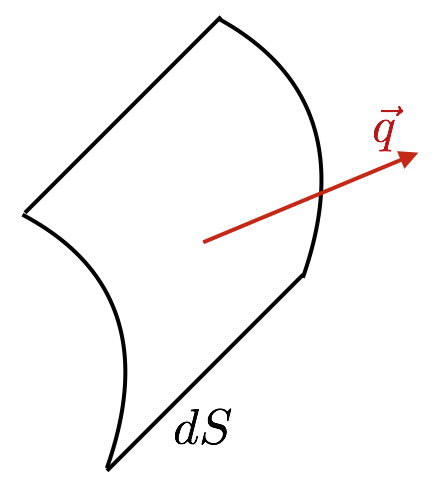
\includegraphics[scale=0.3]{ch1/6}
		\captionof{figure}{}
		\end{wrapfigure}
		For the thermal power expression, we need to introduce a new concept that is the heat flux vector $\vec{q}$ which qualifies a thermal power per unit area leaving the surface. Physically, there is only two heat transport mecanism which are radiation and conduction. Indeed, convection is a specific conduction case where the temperature gradient region becomes thinner and favorises the exchange. The thermal power is 
		\begin{equation}
			\dot{Q} =  - \oint _{S(t)} \vec{q} \vec{n} \, dS = - \int _{V(t)} \nabla \vec{q} \, dV
			\label{eq:1.42}
		\end{equation}
		Replacing the terms of \autoref{eq:1.38} by \autoref{eq:1.40}, \autoref{eq:1.41} and \autoref{eq:1.42} gives 
		\begin{center}
		\theor{
		\textbf{Total energy equation (integral form)}
		\begin{equation}
			\int _{V(t)} \frac{\rho (e+k)}{dt} \, dV + \oint _{S(t)} \rho (e+k)\vec{u} \vec{n} \, dS = \int _{V(t)} \rho \vec{a}\vec{u} \, dV + \oint _{S(t)} (\bar{\bar{\sigma}} \vec{n}) \vec{u}\, dS - \oint _{S(t)} \vec{q} \vec{n} \, dS
		\end{equation}
		}
		\end{center}
		
		The differantial form is obtained using Gauss theorem for the two sides and regrouping all the terms into one integral
		\begin{equation}
		\begin{aligned}
			&\int _{V(t)} \left[\frac{\rho (e+k)}{dt} + \nabla \rho (e+k)\vec{u} - \rho \vec{a} \vec{u} - \nabla \bar{\bar{\sigma}}\vec{u} + \nabla \vec{q} \right] dV = 0 \\
			\Leftrightarrow \qquad &\int _{V(t)} \left[\rho\dot{(e+k)} - \rho \vec{a} \vec{u} - \nabla \bar{\bar{\sigma}}\vec{u} + \nabla \vec{q} \right] dV = 0
		\end{aligned}
		\end{equation}
		
		And considering the fact that this has to be true for all systems, we obtain the two last forms
		\begin{center}
		\theor{
		\textbf{Total energy equation (differential form (1) - divergent form)}
		\begin{equation}
			\frac{\rho (e+k)}{dt} + \nabla \rho (e+k)\vec{u} = \rho \vec{a} \vec{u} + \nabla \bar{\bar{\sigma}}\vec{u} - \nabla \vec{q}
		\end{equation}
		}
		\end{center}
		\begin{center}
		\theor{
		\textbf{Total energy equation (differential form (2) - substantial form)}
		\begin{equation}
			\rho \dot{(e+k)} = \rho (\dot{e} + \dot{k}) = \rho \vec{a} \vec{u} + \nabla \bar{\bar{\sigma}}\vec{u} - \nabla \vec{q}
			\label{eq:1.46}
		\end{equation}
		}
		\end{center}
		Let's finally establish the distribution of the forces in the different energies. If we multiply \autoref{eq:1.36} by velocity $\vec{u}$ and if we observe that $\dot{k} = \frac{\dot{u}_i u_i+u_i\dot{u}_i}{2} = u_i \dot{u}_i$, we obtain 
		
		\begin{center}
		\theor{
		\textbf{Kinetic - Mechanical energy equation}
		\begin{equation}
			\vec{u}\left(\rho a_i + \frac{\D \sigma _{ji}}{\D x_j} = \rho \dot{u}_i\right) \qquad \Leftrightarrow \qquad \rho \underbrace{u_i \dot{u}_i}_{\dot{k}} = \rho u_i a_i + \frac{u_i \D\sigma _{ji}}{\D x_j}
			\label{eq:1.47}
		\end{equation}
		}
		\end{center}
		The difference between total energy \autoref{eq:1.46} and kinetic energy \autoref{eq:1.47} gives the internal energy
		
		\begin{center}
		\theor{
		\textbf{Internal energy equation}
		\begin{equation}
			\rho \dot{e} = 0 + \sigma _{ji} \frac{\D u_i}{\D x_j} - \nabla \vec{q} 
			\label{eq:1.48}
		\end{equation}
		}
		\end{center}
		We see that volume forces only contributes to the kinetic energy, heat flux only to the internal energy and the suface forces to both. 
		
	\subsection{Summary - Complementary equation}
		Let's make the inventory of the 3 substancial equations that we found. How many equations and unknowns do we have? 
	\begin{itemize}
		\item[•] In continuity equation \autoref{eq:1.17}, $\rho$ and $u_i$ are 4 unknowns in 3D. 
		\item[•] In momentum equation \autoref{eq:1.36}, $a_i$ is an external applied force so is known, $\sigma _{ji}$ consists in 6 unknowns (symetric matrix).
		\item[•] In internal energy equation \autoref{eq:1.48}, $e$ and $\vec{q}$ are 4 most unknowns. 
	\end{itemize}			
	\ \\
	The total unknowns number is 14.  The number of disponible equations is 5, 1 thanks to the energy, 1 thanks to the continuity and 3 thanks to the vectorial momentum equation. In this stage, we haven't made any assumption on the nature of the material we're considering. These equations are valid for an elastic solid as a fluid. The main difference is that solids resist to a deformation whereas fluid doesn't. But fluid resists to a rate of deformation. The way that stress tensor $\sigma _{ji}$ is related to the displacement field is called the constitutuve equations. 
	
	\subsubsection{Constitutive relations} 
		For a fluid, the stress tensor depends on the fluid rate of deformation (rate of strain). To express $\sigma _{ji}$, we have to find a quantity in the field of motion of the fluid that represents the rate of strain. If the velocity field $\vec{u}(\vec{x},t)$ was uniform, not depending on $\vec{x}$, the fluid will be moving as a bulk and there is no rate of deformation. The rate of strain must be somehow related to the velocity gradient tensor $\nabla \otimes \vec{u}$. We know that all tensors can be decomposed on an antisymetric and symetric part like 
		\begin{equation}
			\nabla \otimes \vec{u} = \frac{\D u_j}{\D x_i} = \Omega _{ij} + S _{ij} = \frac{1}{2} \left( \frac{\D u_j}{\D x_i} - \frac{\D u_i}{\D x_j} \right) + \frac{1}{2} \left( \frac{\D u_j}{\D x_i} + \frac{\D u_i}{\D x_j} \right).
		\end{equation}
		
		For a constant gradient velocity field, the velocity field is linear in the coordinates
		\begin{equation}
			u_j = \frac{\D u_j}{\D x_i}x_i = \Omega _{ij} x_i + S _{ij} x_i
		\end{equation}
		The first term consists in a pure rotation and does not imply any deformation. Unlike, the second term is the only one that can represent a rate of strain. We conclude that for a fluid, $\sigma _{ji}$ must depend on the symetric part. $S_{ij}$ will be the rate of strain tensor. 